\documentclass{report}

% Packages
\usepackage[utf8]{inputenc}
\usepackage[T1]{fontenc}
\usepackage{lipsum} % Package for generating dummy text, remove it in your actual document

\usepackage{graphicx}
% Commenter un des deux babel
%\usepackage{babel}


\usepackage[french]{babel}
%\usepackage{xspace}


\usepackage{float}

\usepackage{hyperref}
\usepackage{natbib}


\usepackage{tikz-cd}
\usepackage{tcolorbox}

\usepackage[left=3cm,right=3cm,top=2cm,bottom=2cm]{geometry}


% Décommenter au besoin
%\renewcommand{\contentsname}{Table des matières} % Changer le titre de la table des matières
%\renewcommand{\refname}{Bibliographie} % Changer le titre de la section de bibliographie

\title{
    \vspace*{-4cm} % Ajuste la distance du titre par rapport au haut de la 

    \begin{figure}[H]
        \centering
        
\includegraphics[width=0.5\textwidth]{Sources/Logos/Logo_ENSEEIHT.png}
        \label{fig:Logo_ENSEEIHT}
    \end{figure}
    
    % \vspace* permet de forcer l'insertion de l'espace même s'il est en début de page
    \vspace*{0.5cm}
    
    Projet
    
    \vspace{1.3cm}
    
    \textbf{Infrastructure pour le Big Data \& Virtualisation}
    
    \vspace{0.7cm}
    
    {\huge BaDaaS : Big Data as a Service}

    \vspace{1.0cm}

    \begin{figure}[H]
        \centering
        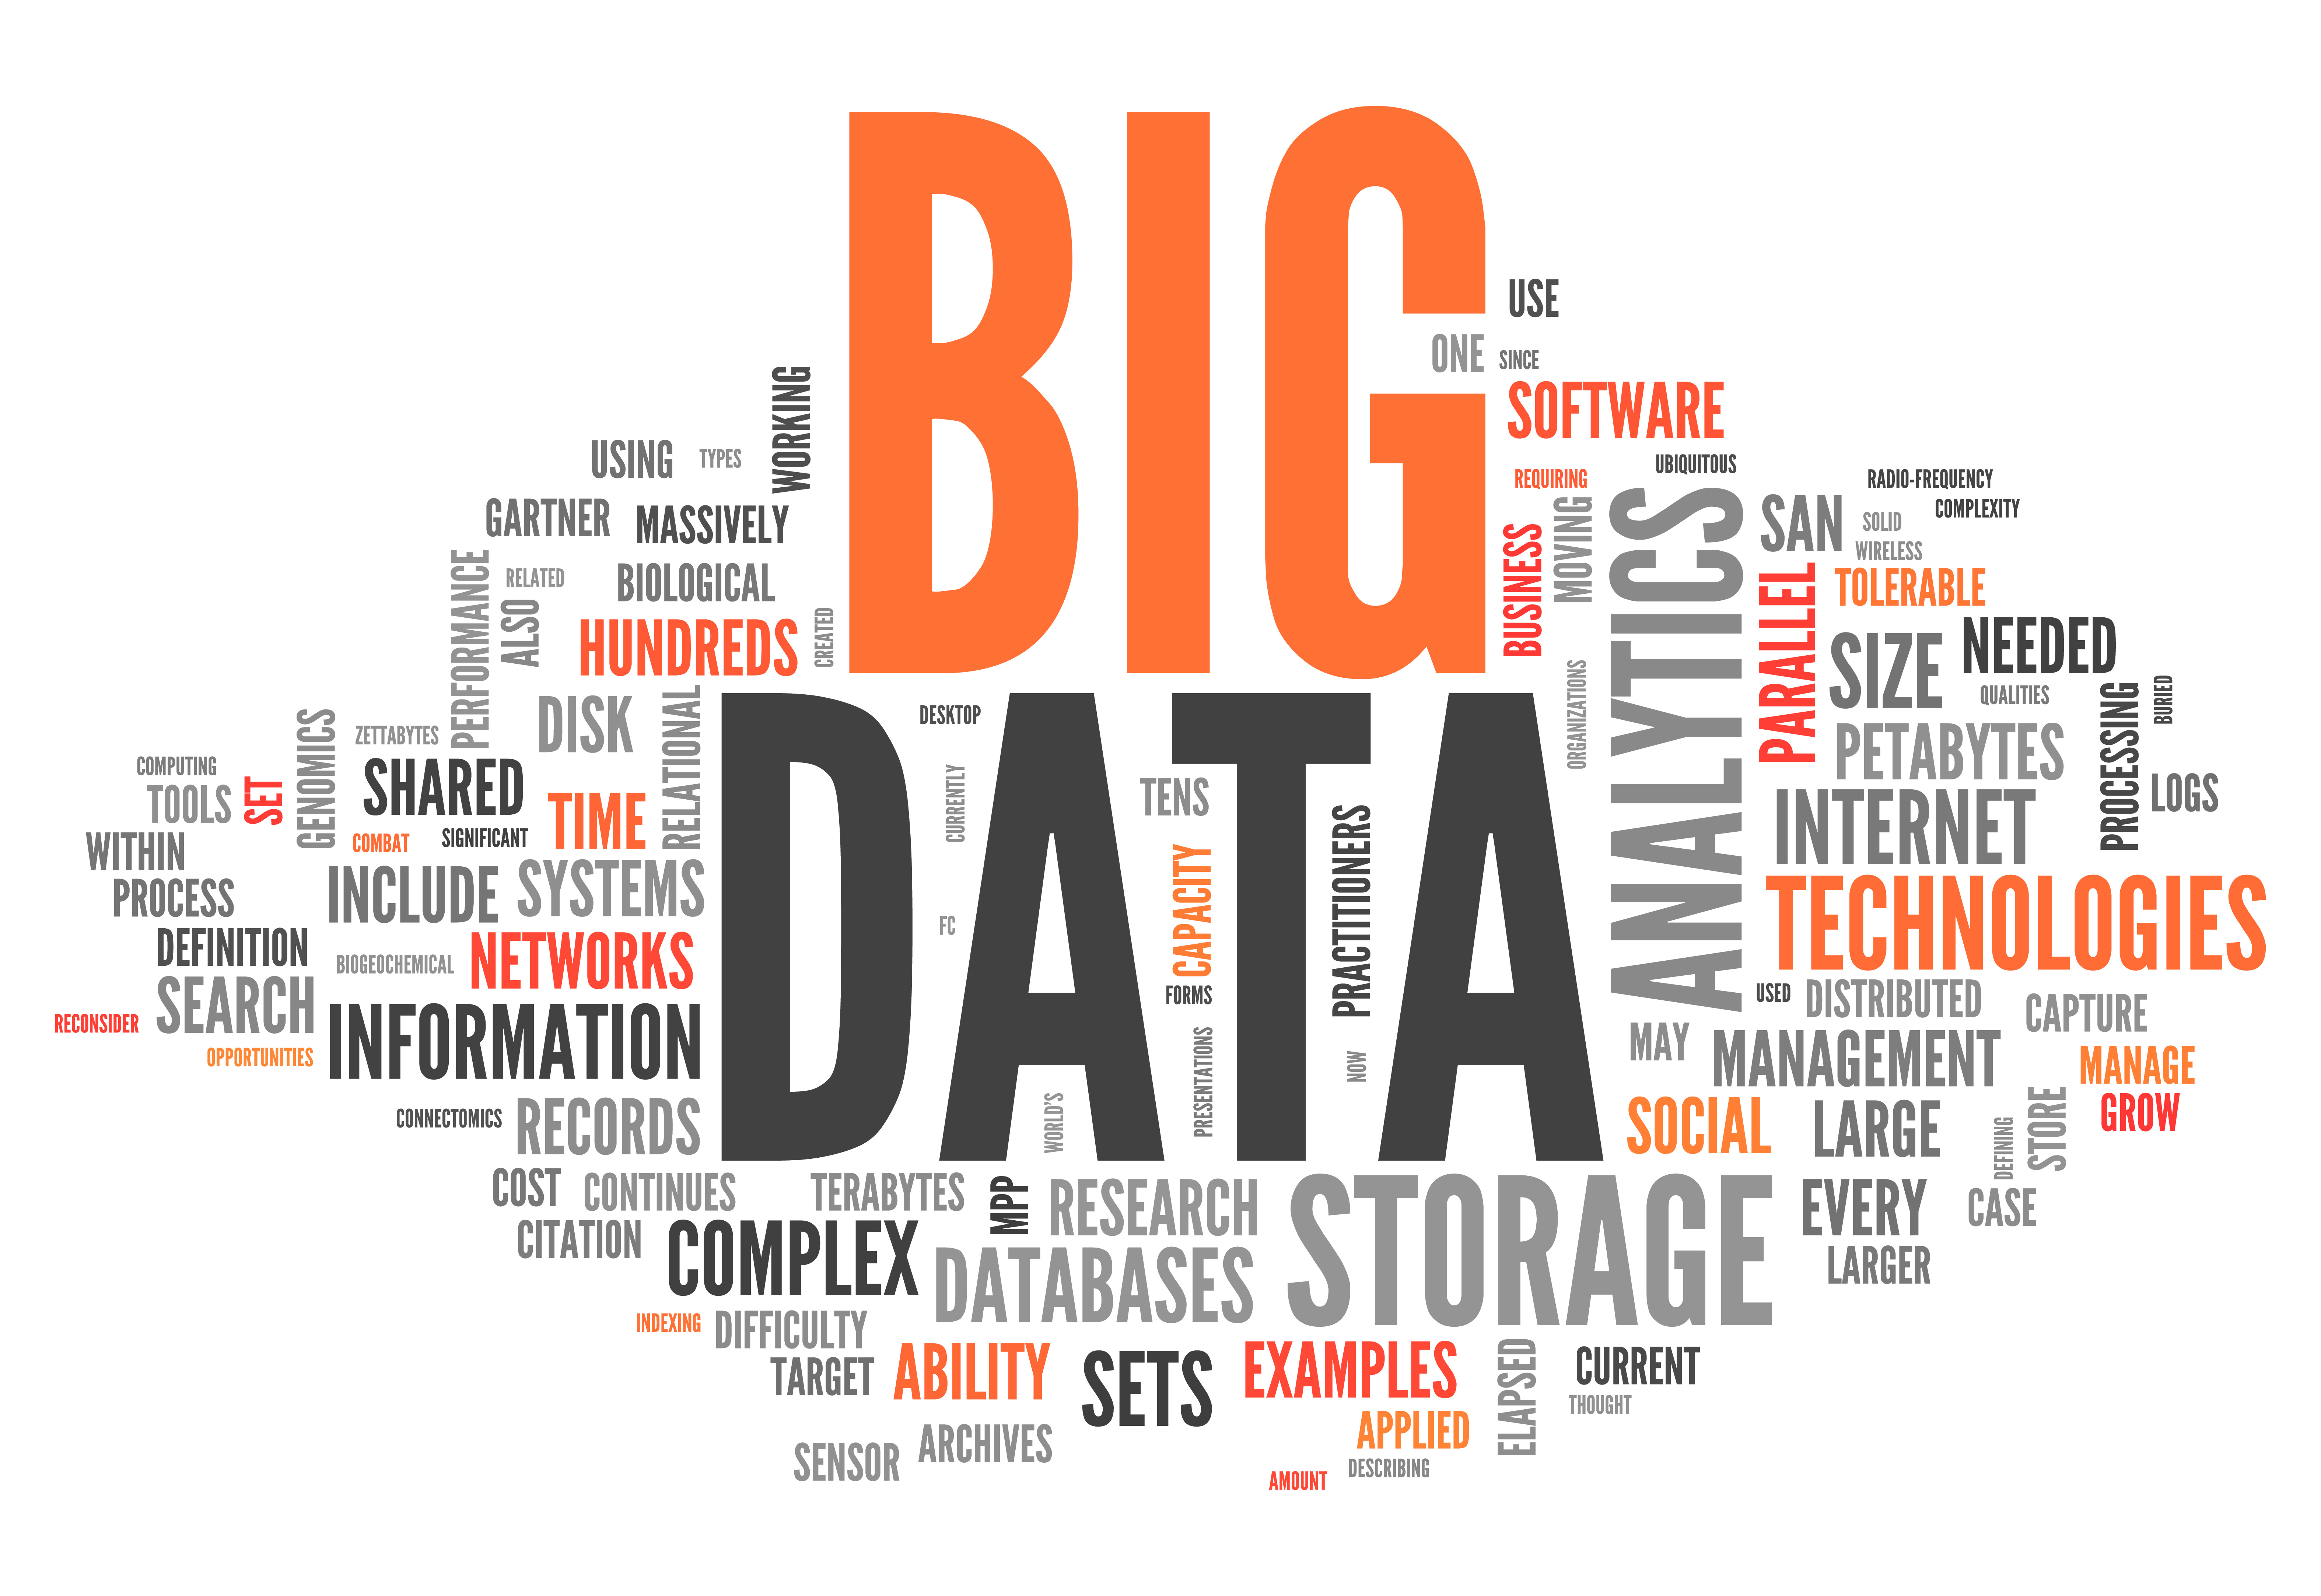
\includegraphics[height=210]{Sources/Couverture/BigData1.jpg}
        \label{fig:Couverture}
    \end{figure}


    % Permet de ne pas afficher les deux lignes (commente un bloc)
    \iffalse
    A thesis presented for the degree of\\
    Doctor of Philosophy
    \fi
    
    {\large \textbf{Thomas Dion - Maxime Moshfeghi - Anh Minh Phung}}
        
    \vspace{0.5cm}
    
    Toulouse INP - ENSEEIHT\\
    France
}




\begin{document}

\begin{titlepage}

% Commande qui affiche le titre défini
\maketitle

\iffalse
\noindent
\begin{minipage}[t]{0.5\textwidth}
    \begin{flushleft}
        \textbf{Auteur :}\\
        \author{Maxime Moshfeghi}
    \end{flushleft}
\end{minipage}%
\begin{minipage}[t]{0.5\textwidth}
    \begin{flushright}
        \textbf{Date :}\\
        \today
    \end{flushright}
\end{minipage}
\fi

% Permet de rajouter le nom/prénom et la date en bas à gauche et en bas en droite, déjà fait avec le title
\iffalse
\noindent
\begin{minipage}[t]{0.5\textwidth}
    \begin{flushleft}
        \textbf{Auteur :}\\
        \author{Maxime Moshfeghi}
    \end{flushleft}
\end{minipage}%
\begin{minipage}[t]{0.5\textwidth}
    \begin{flushright}
        \textbf{Date :}\\
        \today
    \end{flushright}
\end{minipage}
\fi

\end{titlepage}

% N'affiche que le premiers niveaux dans la table des matières (pas les sections par exemple)
%\setcounter{tocdepth}{0}

\tableofcontents % Ajouter la table des matières


\newpage



% Déclaration d'un chapitre factice pour initialiser la numérotation
\chapter*{}

% Réinitialisation du compteur de sections
\setcounter{section}{0}

\renewcommand{\thesection}{\arabic{section}}


\section*{1. Lancement du projet}
\addcontentsline{toc}{part}{1. Lancement du projet}

Dans un premier temps, l'objectif était de créer un réseau de machines virtuelles, réparties sur deux machines physiques. Chaque machine
physique aurait du héberger deux machines virtuelles. L'hyperviseur utilisé était KVM, et nous avons configuré les installations des VM
de sorte à ce que les réseaux aient des adresses distinctes. Voici un schéma simplifié de l'achitecure réseau envisagée :

\begin{figure}[H]
    \centering
    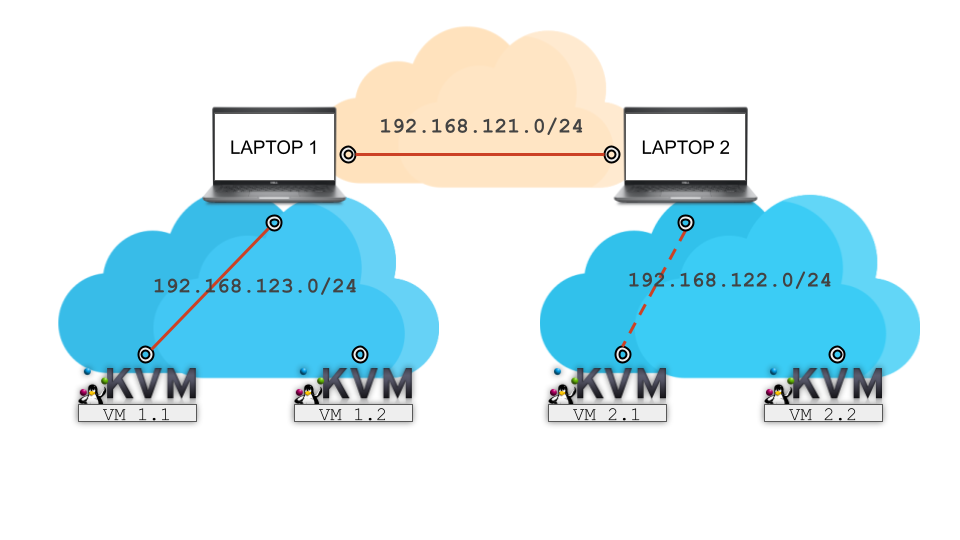
\includegraphics[trim=0 120 0 0,width=1\textwidth]{Sources/Corps/architecture_reseau.png}
    \caption[]{Architecture du réseau envisagé}
    \label{fig:architecure_reseau}
\end{figure}

Malheureusement, il a été compliqué pour la plupart d'entre nous de faire communiquer les VMs de la machine 1 avec celles de la machine 2.
Dans notre cas, nous avions réussi à faire communiquer les VMs de la machine 1 avec la machine 2 (traits rouges pleins sur le schéma), mais
nous n'arrivions pas à communiquer avec les VMs de la machine 2 (peut-être car l'interface physique ethernet et le bridge n'étaient pas
connectées via un "switch virtuel").
Nous avons donc opté pour une architecture ne s'exécutant que sur un ordinateur, avec 3 VMs. 
Voici un schéma de ce nouveau réseau simplifié :

\begin{figure}[H]
    \centering
    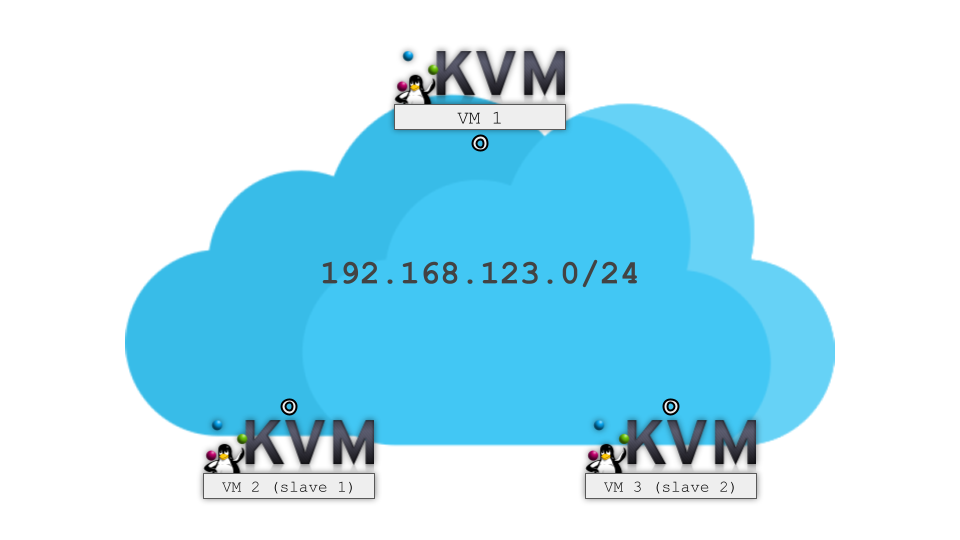
\includegraphics[trim=0 40 0 0,width=0.7\textwidth]{Sources/Corps/architecture_reseau2.png}
    \caption[]{Architecture du réseau réadapté}
    \label{fig:architecure_reseau2}
\end{figure}

L'objectif est alors le suivant :
\begin{itemize}
    \item installer proprement java, hadoop et spark sur chacune des VMs
    \item faire les configurations nécessaires pour déclarer une des VMs comme master, et les deux autres comme slave
    \item exécuter un programme java sur les deux machines slaves depuis la machine master
    \item réussir à créer une interface web permettant de choisir un programme java ainsi qu'un fichier en entrée et un chemin hdfs de sortie
    du traitement, et d'exécuter le programme
\end{itemize}

\newpage

\section*{2. Déroulé et exécution}
\addcontentsline{toc}{part}{2. Déroulé et exécution}
On commence par démarrer le système de fichiers distribué Hadoop. En utilisant la commande start-dfs.sh on va démarrer le processus NameNode, qui gère les métadonnées et les informations de structure du fichier dans HDFS sur le master et démarrer les processus DataNode sur tous les nœuds esclaves, qui stockent les blocs de données réels.\
\begin{figure}[h]
    \centering
    \begin{subfigure}
        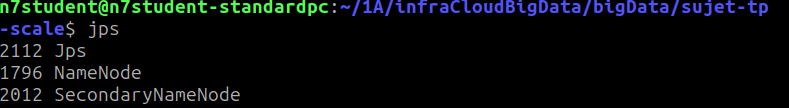
\includegraphics[width=7cm]{JPSstartDFS.png}
    \end{subfigure}
    \begin{subfigure}
        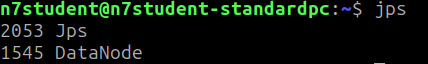
\includegraphics[width=7cm]{JPSstartDFSslave.png}
    \end{subfigure}
    \caption{Processus NameNode/SecondaryNameNode activés sur le master (à gauche) et processus DataNode activé sur les slaves (à droite)}
\end{figure}

Ensuite, on démarre le nœud master de Spark, qui supervise le cluster et gère la distribution des tâches et des ressources et on démarre les nœuds esclaves (workers) de Spark, permettant l'exécution des tâches distribuées par le nœud master.\
\begin{figure}[h]
    \centering
    \begin{subfigure}
        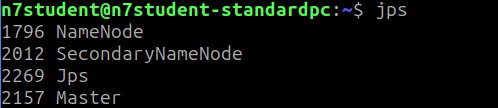
\includegraphics[width=7cm]{JPSstartMaster.png}
    \end{subfigure}
    \begin{subfigure}
        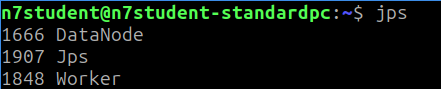
\includegraphics[width=7cm]{Start-Slaves.png}
    \end{subfigure}
    \caption{Processus Master activé sur le master (à gauche) et processus Worker activé sur les slaves (à droite)}
\end{figure}

Enfin, on créer un répertoire dans HDFS vers lequel on pourra transféré des données stockées en local vers HDFS.\

\begin{figure}[h]
    \centering
    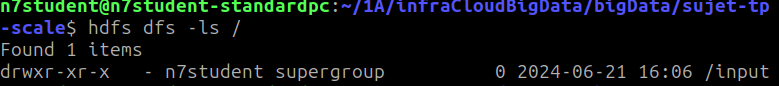
\includegraphics[width=10cm]{HDFS-ls.png}
    \caption{Répertoires présents à la racine de HDFS}
    \label{fig:enter-label}
\end{figure}

Finalement, il suffit de lancer la commande "spark-submit --class <MainClass>  --master <MasterURL> <ApplicationJar>" pour exécuter notre application sur le cluster.\

\vspace{2cm}
\section*{Conclusion}
Au cours de ce projet, nous avons réussi à configurer un cluster de calcul Spark comprenant un nœud master et deux nœuds esclaves sur des machines virtuelles utilisant KVM. Cette configuration nous a permis de distribuer les calculs de notre application.

De plus, nous avons développé une interface graphique pour faciliter l'interaction avec notre application. Cependant, en raison de contraintes de temps, nous n'avons pas pu terminer le développement du backend. 
\addcontentsline{toc}{part}{Conclusion}

%\lipsum[1-2] % Dummy text, remove it in your actual document



\vspace{2cm}

%%Voici une citation \cite{einstein1905}.

%%\newpage

%%\bibliographystyle{plain} % Style de la bibliographie
%%\bibliography{Pages/Bibliographie} % Nom du fichier .bib (sans extension)

\end{document}